%!TEX root = ../Masterthesis.tex
\chapter{System Evaluation}
\section{Camera hardware and control}
The image processing of the camera frames on the Raspberry can be a significant bottleneck for the system. Real-time evaluation demands the processing time of a frame to be in the range of the time of the camera FPS to utilize the full available information from the images. With the current system setup running at 30fps, this means that the image processing time, containing frame readout and downstream processing of the images, has to be done in about $1/30s$ or 33 ms to achieve "real time" processing. Professional stereoscopic setups use cameras with global shutters and a synchronization signal. This enables a sub frame synchronization of the two camera systems. The cameras used in the prototype setup use a rolling shutter instead. Since these cameras are designed to be of easy use for the normal consumer, they lack means of external synchronization. Furthermore, electrical drawings as well as controlling software are closed source. To achieve a from of hardware synchronization, a large amount of reverse engineering would be needed. The multi-layered circuit board of the camera would also complicate the reverse engineering step. As the driver software is closed source, means of getting system information from and to the camera hardware for software synchronization is severely limited. For these reasons, attempting the synchronization of the data further down the processing pipeline is more reasonable.
\\To synchronize the reading start point of both cameras the system boots up to the point where all needed components are initialized. At this point the program waits for a start message from the parent system via UDP. The parent system send the start message at the end of its initialization phase via a UDP broadcast, ensuing that both Raspberry's get the message at the same time.
\newpage
In the normal usage mode,the camera uses mostly automatic modes for parameter setup. This continuous measuring mode showed fluctuation in image brightness and color saturation. To eliminate this problem, all automatic modes are turned of in the camera initialization phase and fixed values are loaded from a JSON file. To get the values for the JSON file a calibration step was implemented into the command line tool. This calibration step enables the user to preview and manipulate the  following values for the camera:
\begin{itemize}
\item Saturation
\item Brightness
\item Gain
\item Exposure time
\item Contrast
\item White balance values for blue and red channel
\end{itemize}
\begin{figure}[H]
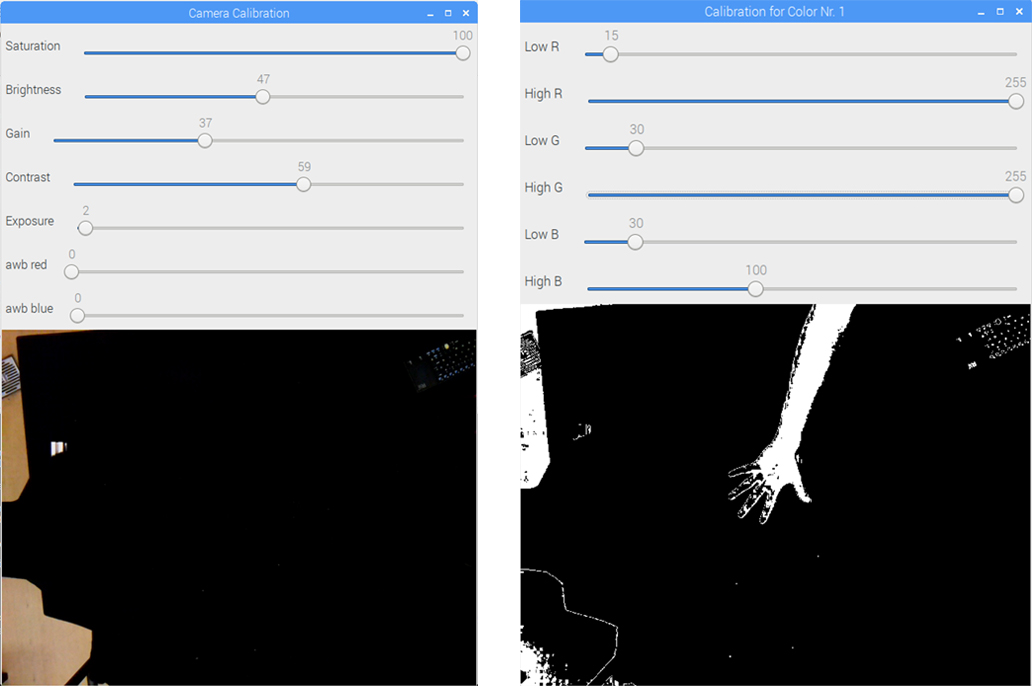
\includegraphics[width=\textwidth]{images/calib_windows.jpg}
\caption{Camera and color calibration utility window}
\label{fig:calibration_windows} 
\end{figure}
The user set calibration values can be written into a new JSON file and are directly loaded into the program after calibration is finished. Control over these parameters is crucial for achieving a constant color separation. \newpage The threshold values values for the color tracking also need to be initially calibrated. These values are dependent on the lighting situation and any change results in the need for re-calibration. To simplify this calibration a calibration function in the same fashion as the camera calibration was implemented.It prompts the user a preview of the resulting thresholded black and white image with applied camera settings. Range sliders for lower and upper boundaries for the three RGB components make it fairly easy to adjust and view thresholding results in real time. The calibration values can also be stored into a JSON file. The calibration values will be fed into the system after finishing and can be saved to a JSON file. This File can be read out on following program startups to eliminate the need of calibration at each startup.
\section{Image processing performance}
The first prototype implementation with \textit{OpenCV} in \textit{Python} showed, that a speed of  33 ms was reachable when only tracking one color. The implementation reached around 30-40 ms processing time when scanning whole images every time. An implementation of an \textit{"Region of interest"} feature  broke down the processing time to around 30 ms for a single color. The downside of the implementation was revealed when implementing the other 4 colors needed to do a full five finger tracking. This approach ramped-up processing time to around 100 ms per frame, making this solution run at 10 FPS.\\ 
The sequential algorithm also showed another design flaw. When not utilizing the ROI approach, the algorithm would scan the whole grabbed camera frame for each color to create the corresponding threshold map. The \textit{OpenCV} color threshold methods are designed to only search for one color threshold at the time, therefore needing this procedure. One solution option is the already mentioned ROI usage. This solution would furthermore benefit from a multi-threaded implementation, as we are not manipulating the original image. Parallel memory readout is not a problem and the generated mask can be saved separately.\\
Another approach which could help speed up the process is implementing an own method for thresholding the grabbed frame with the possibility to do all the needed color thresholds in one image loop. With this solution, the overhead would be reduced by 4 image iterations, thresholding operations would stay the same as these still have to be run on each pixel. The output of this method would then return the 5 needed threshold mask for further processing.\\
A second performance issue that arose from the first prototype was that the input camera frames came RGB coded. For better options of color separations, the image was initially converted into HSV colorspace. This operation turned out to be second longest operation after frame grabbing. \\Testing of the cameras showed that the color segmentation in the original RGB images of the cameras are good enough for the used test colors, causing this step to be omitted and shaving off several milliseconds of processing time.
The rest of the processing steps were lying in the sub millisecond range and are therefore not as valuable for performance optimization.
The results from this prototype showed, that the \textit{OpenCV-Python} combination is not suitable for reaching the 30 ms target time. The OpenCV library used by python is actually just the ported version of the C code library with bindings for python. As \textit{C} and \textit{C++} are more hardware near and therefore more performant, the second prototype implementation was done in \textit{C++}.
%\begin{table}[ht]
%\centering
%\caption{Speed measurements for the used implementations}
%\label{Speed measurements for the used implementations}
%\resizebox{\textwidth}{!}{
%\begin{tabular}{|l|l|l|l|l}
%\cline{1-4}
%Timings in ms        & \begin{tabular}[c]{@{}l@{}}Python Single Thread \\ without ROI\end{tabular} & \begin{tabular}[c]{@{}l@{}}C++ Single Thread \\ without ROI\end{tabular} & \begin{tabular}[c]{@{}l@{}}C++ Single Threadpool \\ Thread with ROI\end{tabular} &  \\ \cline{1-4}
%Frame Reading        &                                                                             &                                                                          &                                                                                  &  \\ \cline{1-4}
%HSV Conversion       & \multicolumn{1}{c|}{50.852}                                                 & \multicolumn{1}{c|}{41.125}                                              & omitted                                                                          &  \\ \cline{1-4}
%Image Blur          &                                                                             & \multicolumn{1}{c|}{147.239}                                             & 
%varies with ROI size &  \\ \cline{1-4}
%Mask erode/dilate   &                                                                             & \multicolumn{1}{c|}{165.663}                                             & varies with ROI size &  \\ \cline{1-4}
%Color Threshold      &                                                                             & \multicolumn{1}{c|}{14.686}                                              &                                                                                  &  \\ \cline{1-4}
%Position Calculation &                                                                             &                                                                          &                                                                                  &  \\ \cline{1-4}
%                     &                                                                             %&                                                                          &                                                                                  &  \\ \cline{1-4}
%ROI Readout          &                                                                             &                                                                          &                                                                                  &  \\ \cline{1-4}
%\end{tabular}}
%\end{table} The usage of \textit{C++} as the programming language provides more control over memory management and therefore reduces unnecessary memory data copies as these can be handled by pointers to memory locations.\\
\\The ported version of the Python code to\textit{ C+}+ initially showed similar performance measurements when using the sequential approach. This was to be expected, as it is the same code the python bindings are using. Further investigation into code timings showed, that another bottleneck was the image optimization feature which applied erosion and dilation operations to remove high frequency noise in the image. This operation brought the time up to 100 ms processing time when processing the whole frame area, making the algorithm  not usable for "real time" application. \\Removing this feature brought a major speed up in processing time. 
Furthermore, the implementation of a thread pool, which handles all the color detection jobs, brought down the calculation time for 5 colors to around 120-140 ms. Although these times are still not usable for real time, it brought a significant performance boost.\\
A test with lower resolution than 640x480 showed that the calculation time can be  reduced furthermore. This indicated that the ROI idea would be feasible for  further performance optimization. A test at a frame resolution of 320x240 pixels reduced the processing time for all five colors to below 10 ms.\\
\begin{figure}[H]
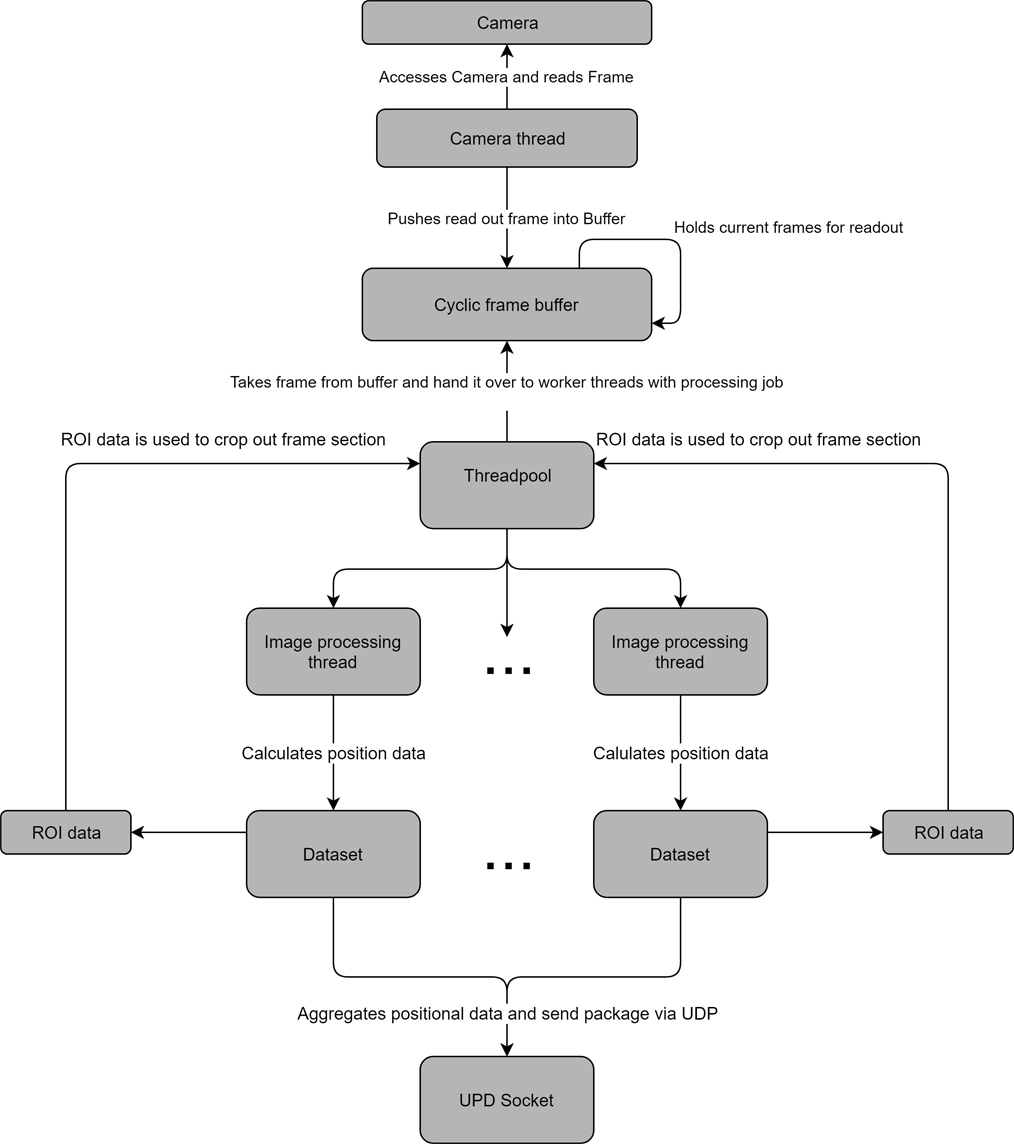
\includegraphics[width=\textwidth]{images/pi_workflow_500.jpg}
\caption{Work flow of the C++ implementation with thread pool solution and ROI for high framerate solutions}
\label{c++ work flow map} 
\end{figure}
Utilization of the knowledge from these tests led to the implementation of the aforementioned\textit{ "Region of interest"} feature (see Figure \ref{c++ work flow map}).
The first frame is analyzed as a whole frame, optimally resulting in the detection of a marker. As the marker detection creates a rectangle around the tracked area, we already have the coordinates for the ROI and only have to add an offset to this area.
\\The value of the offset has to be set high enough to ensure that in the following frame, the tracking marker is still contained in the ROI. It also has to be ensured, that the generated ROI is clamped to the frame dimensions. If not doing so, parts of the readout are can be located outside of the image plane, causing readout errors when used for the subsequent frame. The following frames will then be processed with the input of the ROI, selecting only the defined section of the image and updating the ROI with the new data for that frame.\\
Performance measurement for tracking consistency with stationary color trackers was performed for a time period of 10.000 frames to get qualitative results. The sequential implementation with the usage of the ROI showed an average processing time of 46 ms with a standard deviation of ~11 ms.\\
Further analysis showed that the high standard deviation came from peaks in performance times that took up to 400 ms when loosing tracking. Filtering all values over 50 ms out from the data set showed that only $1\%$ ($\sim 1000$ out of $10.000$ frames) of the recorded processing times were lying outside of this time frame. Filtering out these values form the data set and recalculation dropped the average processing time down 3 ms to around 43 ms. The standard deviation of was dropped drastically from its previous 11 ms to around $1.6$ ms. This shows that a filtering of processing times on the Raspberry can lead to a more consistent frame processing time. To do so,after every processing cycle the time needed is checked and if it is over the defined time limit,no data should be sent.\\
Since this performance measurement does not show which part of the process consumes large amounts of processing time, the same measurement was done with a finer time tracking on the single parts of the processing pipeline.
\begin{table}[H]
\centering
\caption{measurement results for sequential processing timing measurement}
\label{tbl:sequential_performance_values}
\begin{tabular}{|c|c|c|c|c|c|}
\hline
\begin{tabular}[c]{@{}c@{}}Time \\ in ms\end{tabular} & \begin{tabular}[c]{@{}c@{}}Image \\ retrieval\end{tabular} & \begin{tabular}[c]{@{}c@{}}Stereo \\ rectification\end{tabular} & \begin{tabular}[c]{@{}c@{}}Color detection\\ (6 colors)\end{tabular} & \begin{tabular}[c]{@{}c@{}}UDP \\ sending\end{tabular} & \begin{tabular}[c]{@{}c@{}}Summed \\ time\end{tabular} \\ \hline
Average                                               & 0.91685                                                    & 31.39436                                                        & 14.55122                                                             & 0.12053                                                & 46.96780                                               \\ \hline
Std.Deviation                                        & 0.17105                                                    & 7.19069                                                         & 5.06205                                                              & 0.06031                                                & 10.77171                                               \\ \hline
\end{tabular}
\end{table}
Table \ref{tbl:sequential_performance_values} highlights the performance bottlenecks of the system. Image retrieval from the camera as well as the time to process and send the data results via UDP are in the sub millisecond range, therefore they impose no significant delay. Without these two steps, the remaining 96\% of the processing time is taken up by the image stereo rectification and the color tracking.When comparing these two, the far larger time consuming part is taken up by the stereo rectification part with nearly two thirds of the processing time.\\
Stereo rectification is usually done to ensure that the two used images have an aligned horizontal orientation. This is needed for camera pairs that are not aligned horizontally and/or parallel. Since the camera setup ensures that the cameras are aligned parallel and at the same horizontal height, the rectification step can be omitted for performance reasons. It cuts down 67\% of the processing time of the system. As the stereo calculation does not use the vertical position difference for calculations, the possible resulting differences can be dealt with via filtering on the receiver side.
A solution for the color tracing time improvement was already described before. Utilizing a multi-threaded approach could lead to further reduction of the processing time. A comparison between the before mentioned sequential algorithm and a multithreaded implementation was tested as well. The multi-threaded implementation was designed to run the same processing stack as one loop of the sequential approach on each thread. Measurements over 10.000 Frames for stationary as well as moving targets were made. One camera was run with the sequential implementation while the second one ran the multi-threading approach parallel. Thereby it is ensured that both cameras have the same measurement conditions.

\subsection{Color accuracy and ROI size}
As already mentioned in the conceptional phase, the lighting of the tracking area is a major factor. Variations of lighting intensity and color temperature cause the color of the trackers to shift their color. This can cause a fluctuation in the calculated tracker positions, as the defined color threshold ranges are kept as small as possible to achieve a clean separation of the tracker colors and reduce unwanted noise. \\
System testing with the 5 different colored shrink tubing markers showed, that the color tracking for colors outside of the color range of the human skin tones (green,blue) is rather unproblematic. The color markers falling into the colorspace of posible light reflection from skin may cause probelms, dependng on the lighting situation of the setup.
\begin{figure}[H]
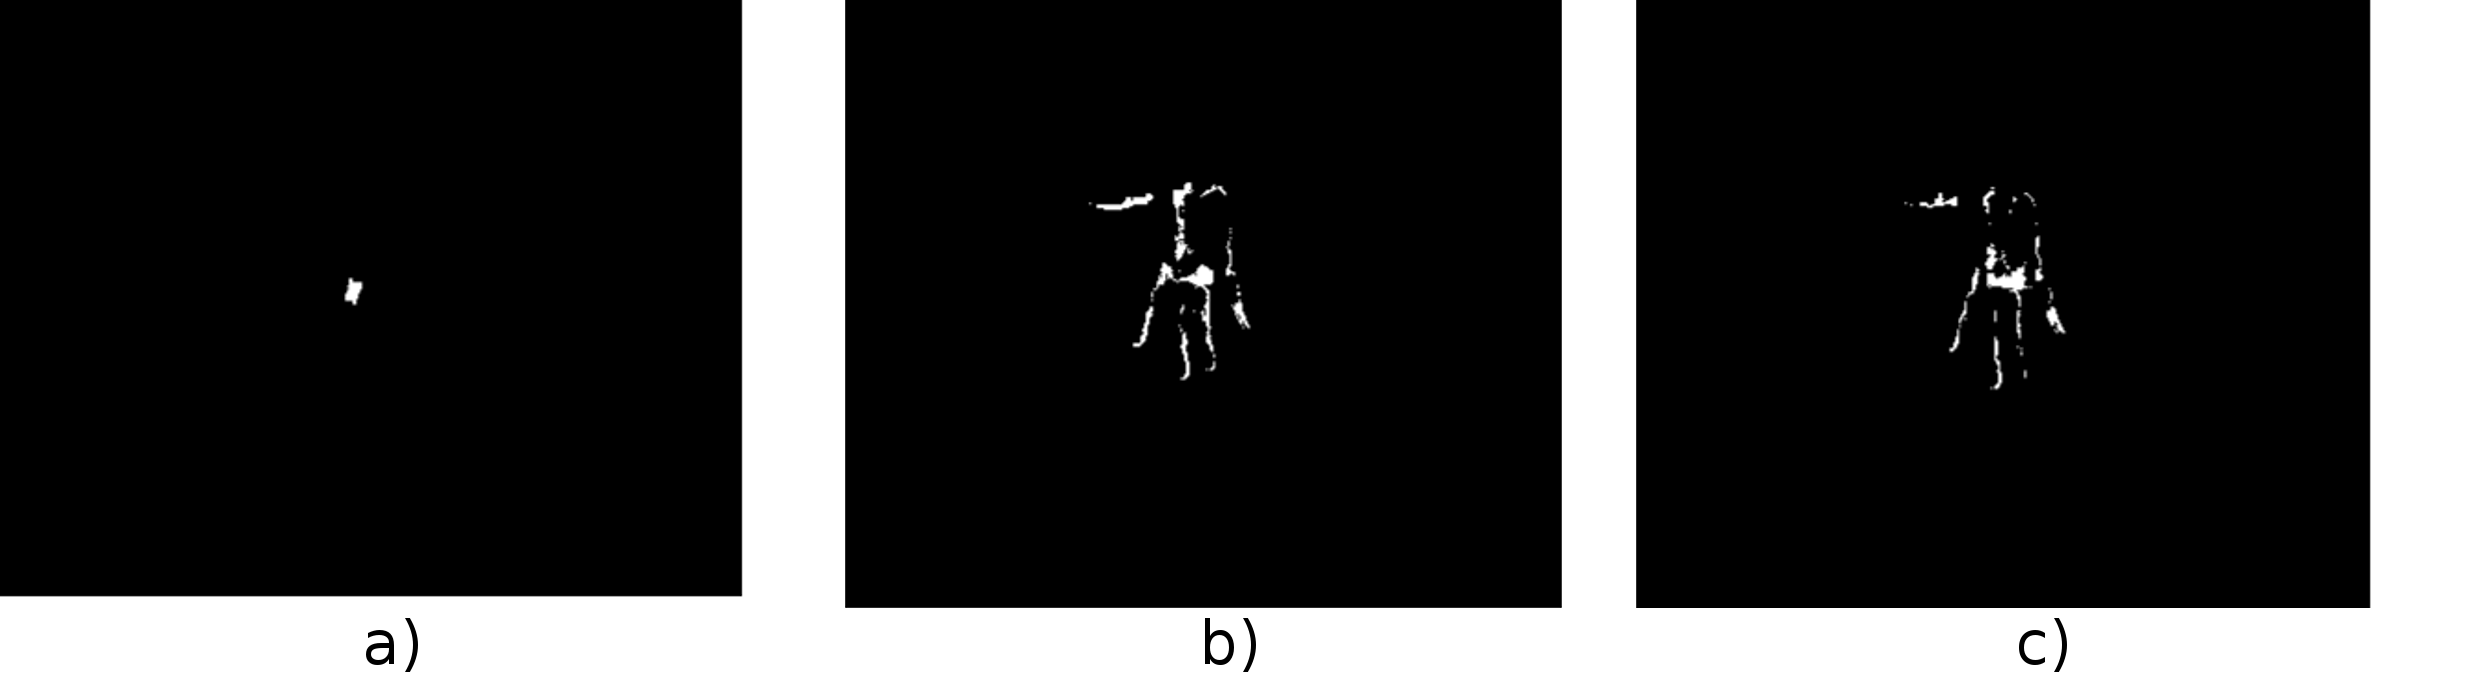
\includegraphics[width=\textwidth]{images/color_tracking_probs.png}
\caption{Images showing reflection problems with  orange color thresholding. a) Correct threshold with only the marker being thresholded b-c) Depending on the rotaton of the hand, skin reflecton color falls into tracking threshold.}
\label{img:Color_reflecton_problems} 
\end{figure}
Figure \ref{img:Color_reflecton_problems} displays such a case where depending on the orientation of the hand, refletion from the scenery lightng can fall int the color tone space of the tracked marker, causing large parts of the hand to light up in the image. Since the calculation of the trackng marker position relys on finding the largest closed "white" area in the thresholded image, this can cause a "jumping" of the calculated position. 
\\The first solution for this problem is to narrow down the color threshold spans. By doing so, one can ensure that only the wanted colors are tracked. This method does have a downside effect. When the markers are moved in the tracking space, light variations and shadowing will cause the colors to shift their appearance slightly. With broader threshold ranges, this does not seem to be a large problem as these changes still lie inside the ranges. Narrowed down color ranges might not include these color variations, creating cavities in the thresholded image.\\ The applied morphological operations on the image can fix these problems up to a certain point, depending on filter kernel size, but for larger areas this could vary position tracking results.\\\\The implemented ROI feature speed up the whole system calculations once the colors are found. Before this point, the system scans whole frames to find colors, which takes more time than the much smaller ROI regions.
Empirical evaluations showed, that for the used tracking space, a ROI region size offset of 40 px in x and y directions produces the best results in terms of consistency. Smaller region offsets caused the system to use tracking for faster hand motion, which causes system slow down until the tracking has recovered. Generally, larger ROI's produce more constent tracking results at the cost of higher calculation time.
\subsection{Finger markers}
\begin{wrapfigure}[16]{r}{0.3\textwidth} 
\centering
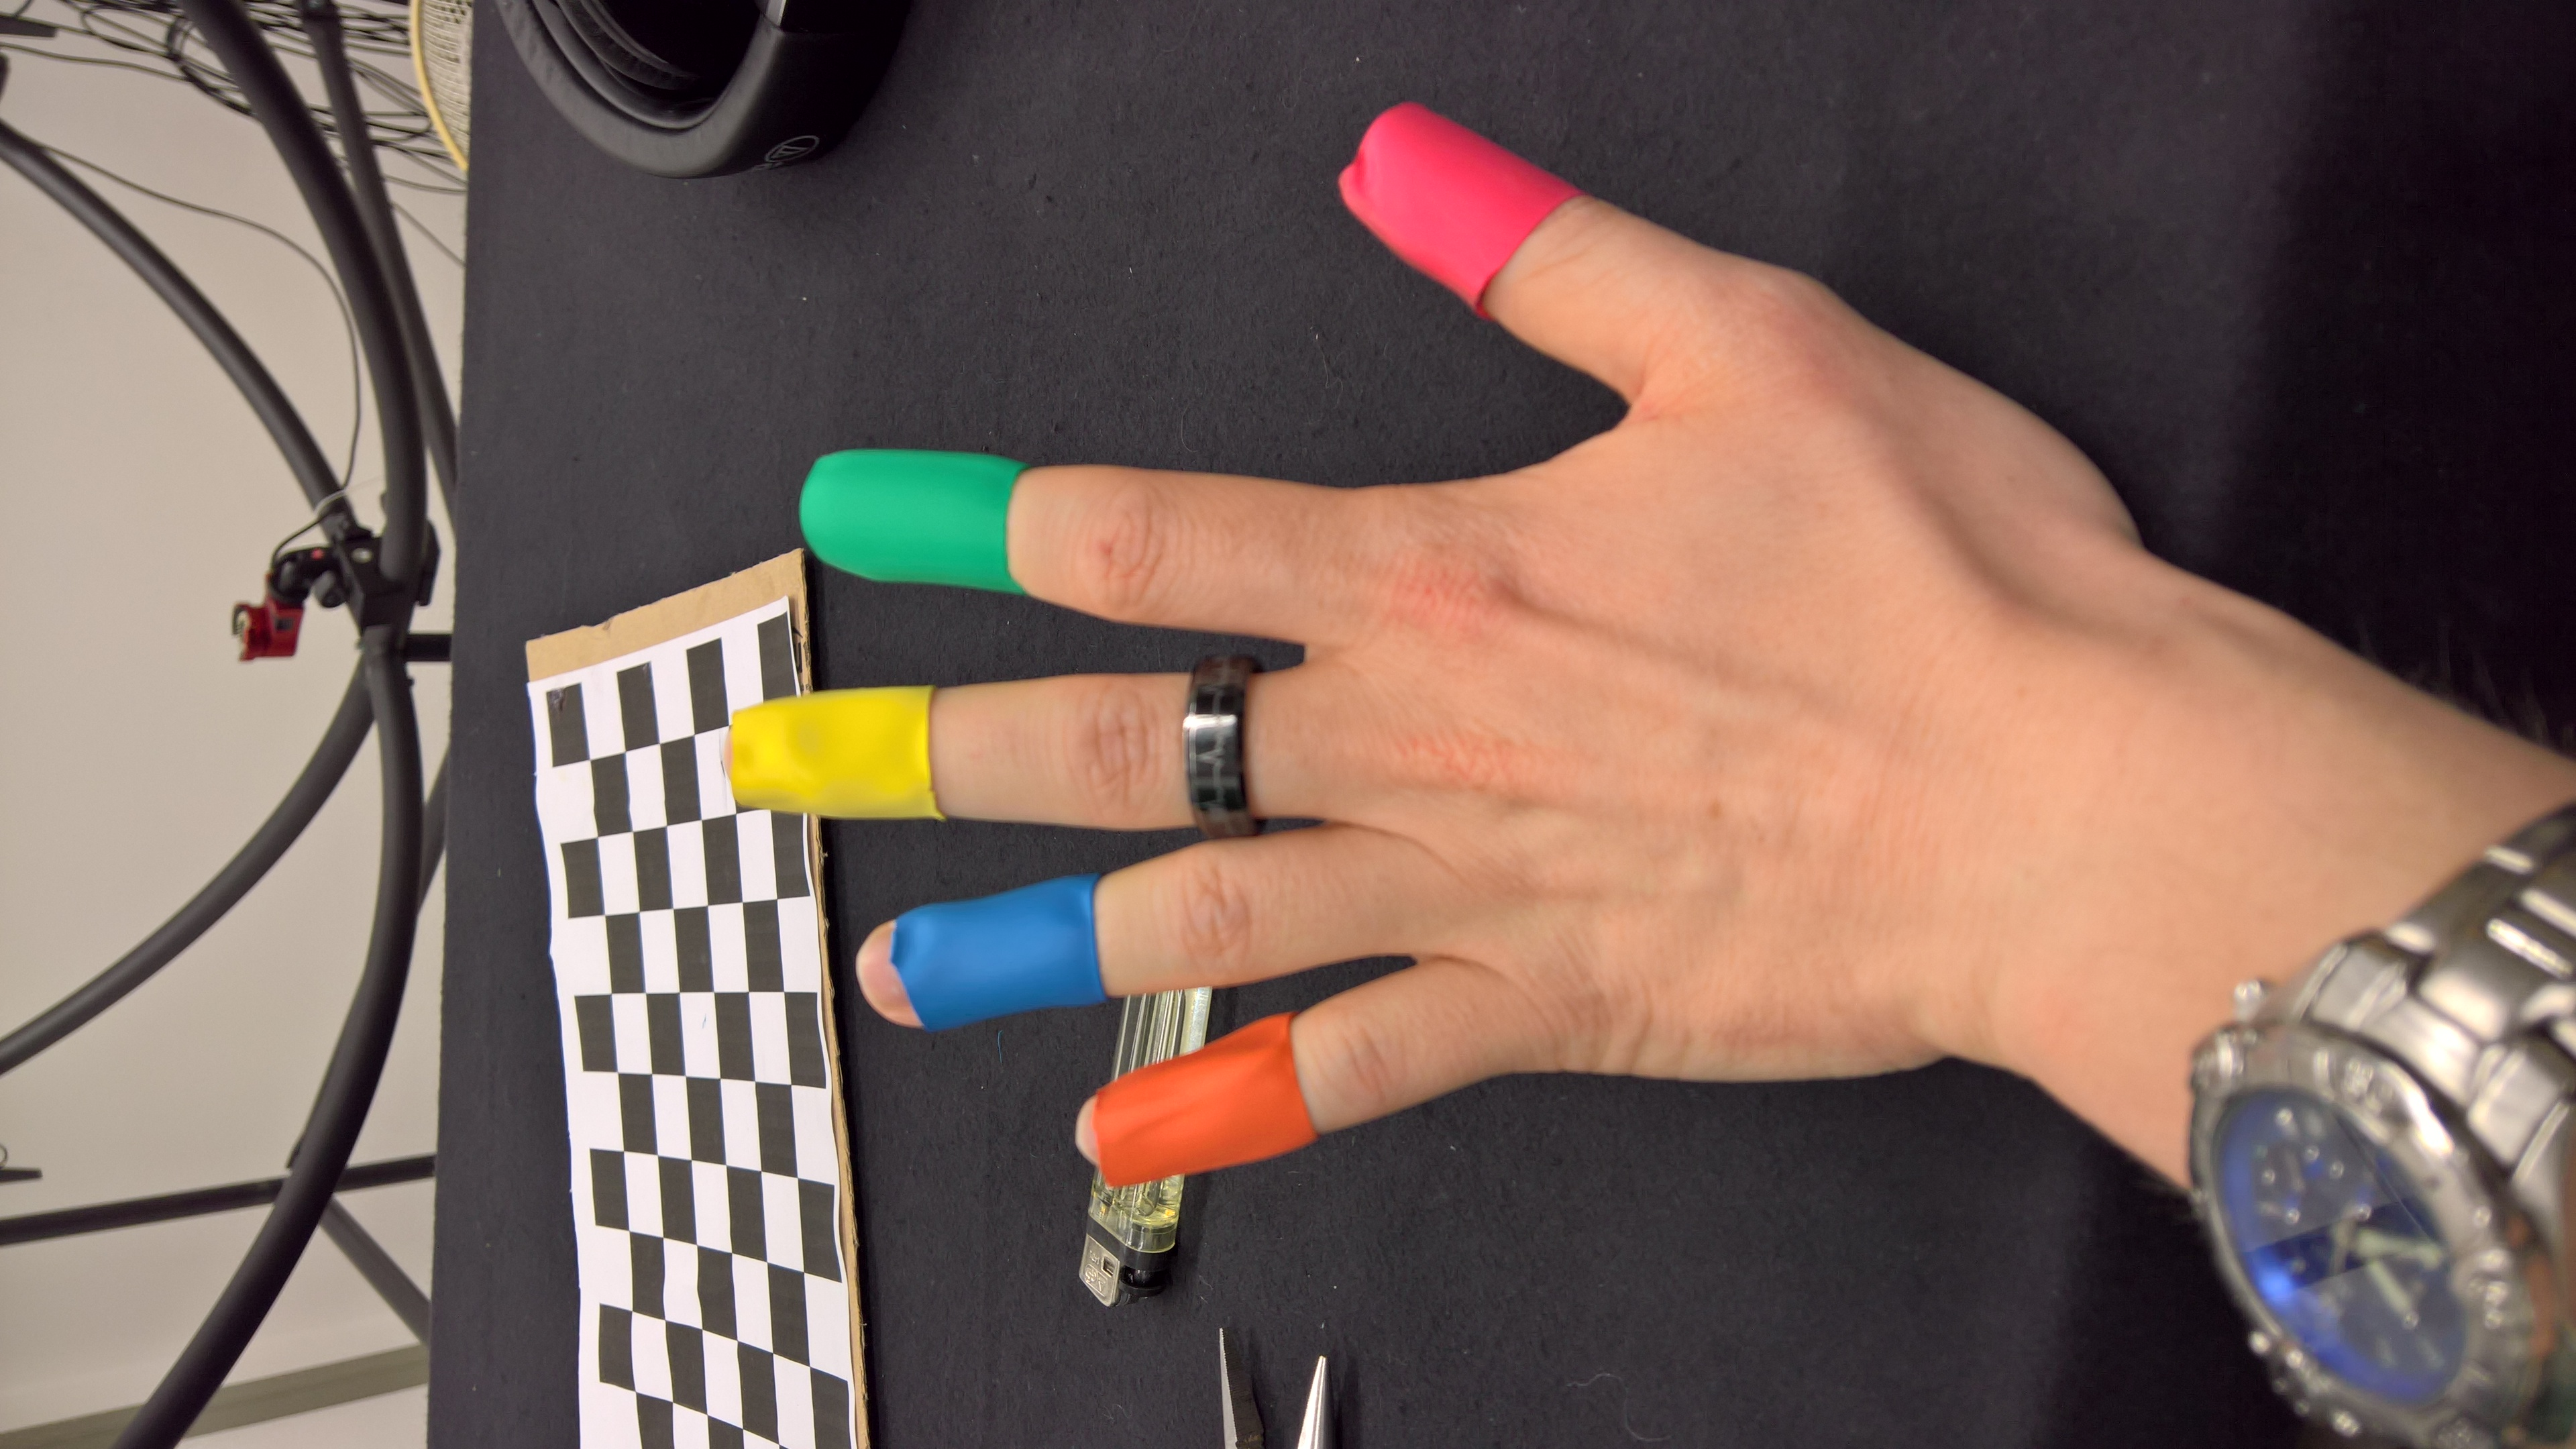
\includegraphics[width=\textwidth/2,angle=-90]{images/color_markers_hand.jpg}
\caption{First set of shrink tube color markers }
\label{img:first_set_color_markers}
\end{wrapfigure}
The initial color marker size was selected to be relatively large, spanning most of the last segment size of each finger.
The used material of the colored shrink tubing was selected because it seemed to be relatively diffuse and therefore unprone to errors resulting from the reflection of the scene lighting. The material turned out to be mostly diffuse reflecting, but depending on color and angle of light incidence, reflections in the color of the scene light did occur.
A test set of smaller marker was also evaluated, showing similar tracking results in comparison to the larger markers and also the same color reflection problems.\\The benefit of a smaller marker size would be much lower restriction of the finger movements and also unveiling the fingertips of the fingers for better haptic interaction.
As both markers showed the above described problem of mixing marker area with possible skin reflections, and improvement to the markers was applied. At both ends of the larger markers, a piece of gray colored tape was applied to create an artificial border for the tracking algorithm.
\begin{figure}[H]
\centering
\includegraphics[width=\textwidth/2]{images/small_and_improved_markers.jpg}
\caption{Improved larger and smaller set of shrink tube color markers }
\label{img:second_color_markers}
\end{figure}
The idea behind this solution was to create a fixed border between the color area of the tracker and the color area of the skin tones. The grey color of the border ensures that this area will not be tracked. The usage of black instead of gray would even furthermore ensure this. 
\\Since the threshold algorithm searches for the largest closed color area in the binary threshold image, this border should cause a separation of unwanted skin reflection area and actual tracker color area. The problem that the resulting color marker area might not be the largest area still persists after this improvement, but this case has to be handled separately.
\\Optical results showed that for the colors lying outside of the red to orange color spectrum that skin reflections produce, the artificial border stabilized the color detection.
\\The idea of using shrink tubing as marker material showed to be suitable except in the cases described above. One downside of the material is that the displayed colors are already the highest variety of available colors on the market. Other colors from the green and blue color areas like purple are simply not available or have to be ordered as a special request in larger amounts.
\\Also the original diameter is much larger than a human finger. The used shrink tube is able to be shrunk to one third of its size. The reason for this was to be able to adapt to the varying diameters of the human hand. The shrinking procedure requires a constant amount of heat to be applied to the material to activate the shrinking. The amount of heat that is needed surpasses the heat production of a standard hair dryer since the original application of shrink tubing is on heat resistant cables. The heat that needs to be applied can easily be more than 100 degree Celsius, which makes a direct application on the users hand highly insecure.
\\\\For the prototype, the shrink tube parts were shrunk with a standard cigarette lighter and continuously fitted onto the user finger until the desired form was reached. This method showed to  be sub optimal, since the flame of the lighter produces only a punctual heat source. This caused uneven shrinkage of the heated parts. This can lead to cavities or bumps in the material and change the reflection properties at these points. A regulated heat gun would probably generate better results.
\\To get smoother shrinking results, parts of PVC tubing with the correct diameter could be used as dummy parts for the main part of the shrinking.\\
\\Another approach that was tested was the usage of matte acrylic paint to cover parts or even the whole finger. The matte acrylic paint comes with the benefits of being easily to apply to the finger. Acrylic paint is available in much more color variations than the shrink tube. The finger coating is dry in under a minute after application. Adaption for finger size is automatically included in the application process. If the tracking system does not need to evaluate for hand rotation, i.e. the working principle is a top on view, a nail polish style application of the color on the fingernail can be sufficient for the tracking system. The thumb needs to be treated separately, as it has more rotation capabilities than the other fingers. The thumb should be marked completely on all sides to achieve a constant tracking. If hand orientation is tracked, the other fingers should be completely marked as well.
\begin{figure}[H]
\centering
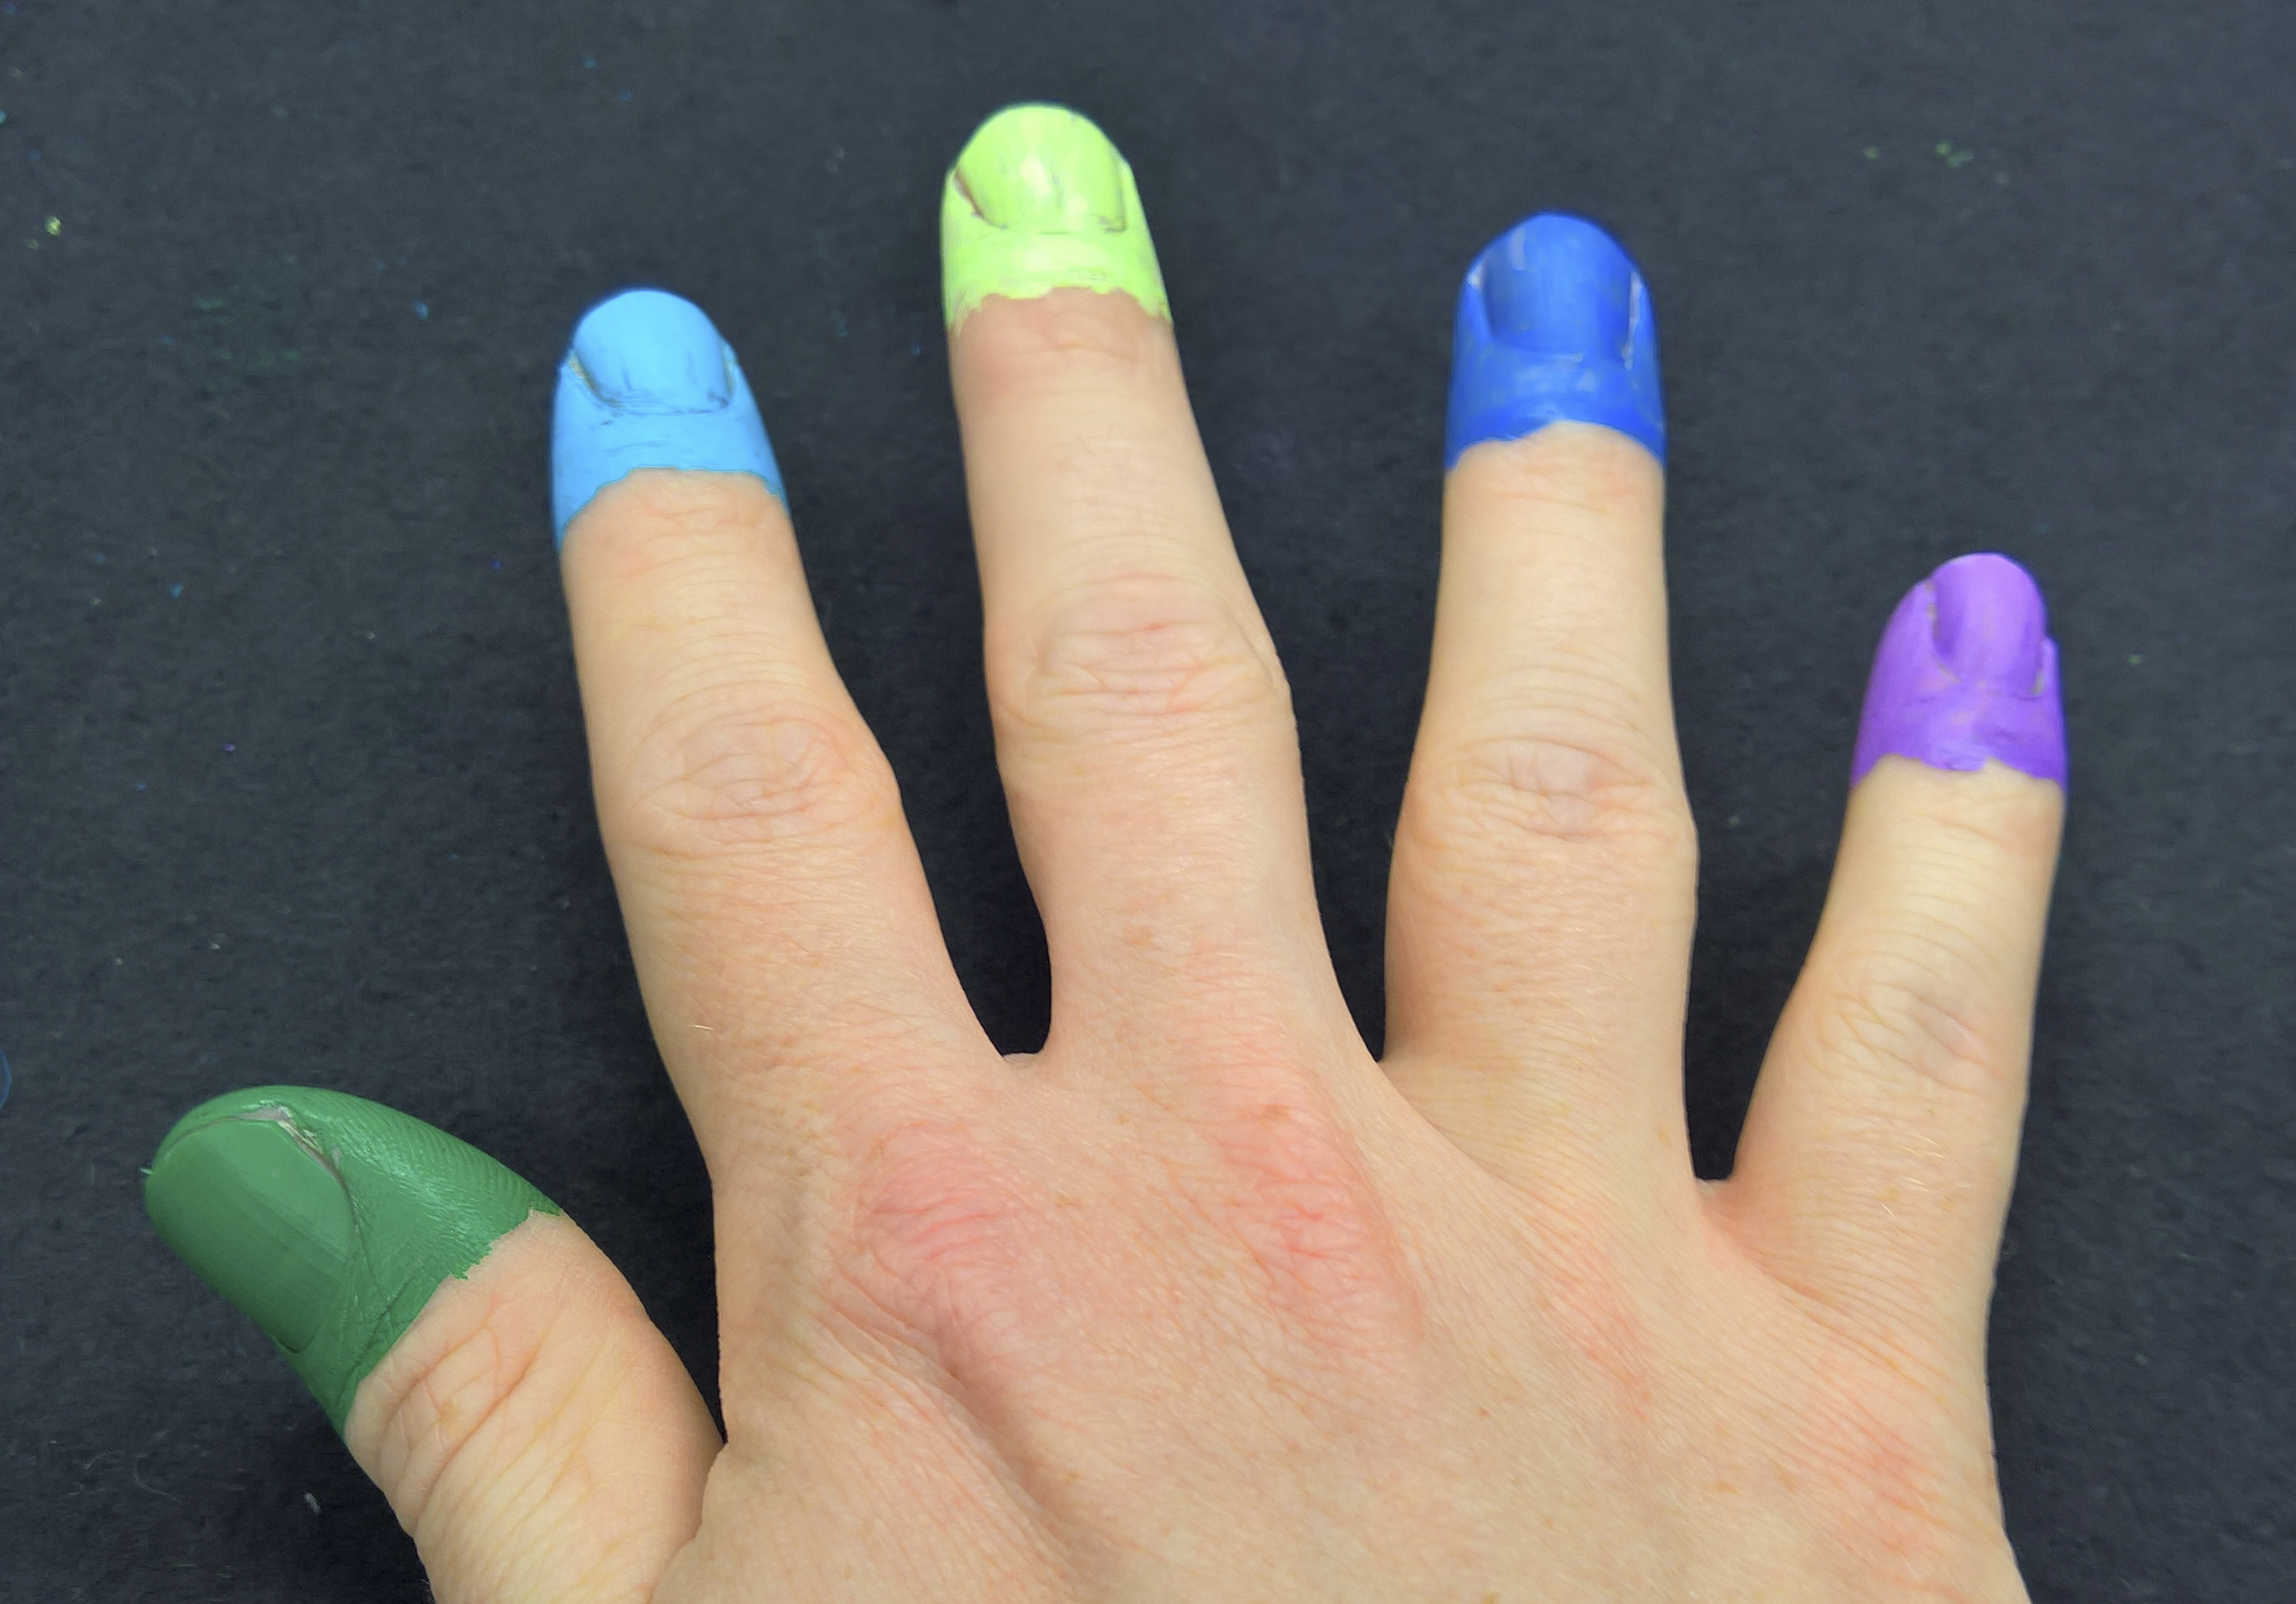
\includegraphics[width=\textwidth/2]{images/final_finger_markers.jpg}
\caption{Finger marked with suitable acrylic colors}
\label{img:final_markers}
\end{figure}
\todo{measure new marker}
The best tracking results in terms of stability and color separation were achieved with the acrylic paint as marker material. For the colors a mixture of blue and green color tones together with red tones in the purple and magenta section were chosen as the final colors.
\begin{figure}[H]
\centering
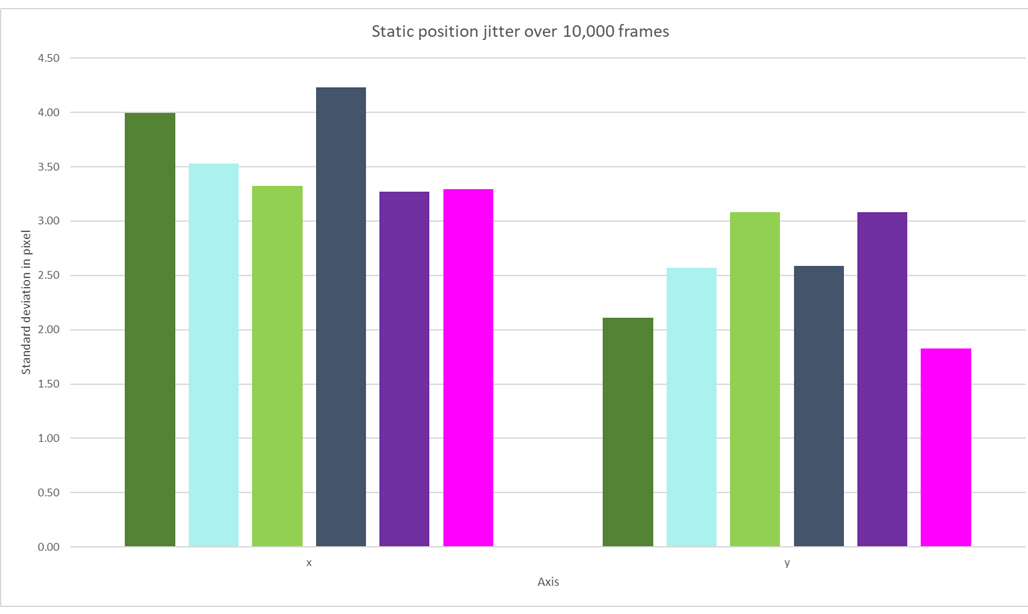
\includegraphics[width=\textwidth]{images/acrylic_color_jitter.jpg}
\caption{Bar chart showing postion jitter of final colors in static position}
\label{img:color_jitter}
\end{figure}
\todo{Measurements} The usage of the acrylic color also provides the least degradation in terms of gripping haptics on the fingers. Figure \ref{img:color_jitter} shows the measured static position jitter of the system with the final colors. The reachable sytem precison lies between 2 and 5 pixel deviation. At a system resolution of 640x480 pixels, this results in a deviation of $\sim 0.7\%$ on the x axis and $\sim 1.0\%$ deviation on the y axis.
\subsection{Depth measurement accuracy}
To determine the accuracy of the system for it's depth measurement values a simple test bench setup was used. The camera rig was aligned horizontally and fixed to the test bench. A large sized colored marker (75 mm x 50 mm) was used as target for detection. The marker marker was positioned at altering distances from the camera rig along the central axis of the camera rig. The height at which the camera rig is positioned in the experiment setup will be around 100 cm, so the measured distances started at 100 cm from the camera and were decremented in steps of 5 cm until 20 cm in front of the Camera Rig(see Appendix Table \ref{Depth measurement Values} and Figure \ref{char:DisparityToDistanceChart}).\\
\begin{figure}[H]
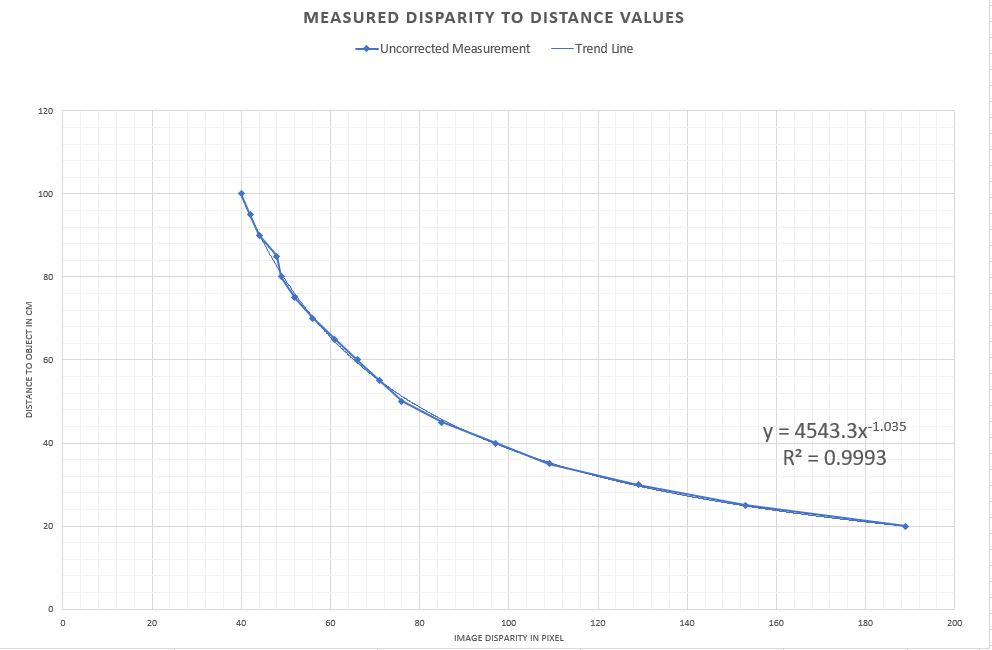
\includegraphics[width=\textwidth]{images/Disparity_to_distance.JPG}
\caption{Chart showing the results of the disparity measurement with a plotted trend line}
\label{char:DisparityToDistanceChart} 
\end{figure}
The accuracy of the camera system is limited by the number of pixels in relation to the camera view angle\cite{JernejMrovlje.2008}:\\
\begin{equation}
\Delta\varphi=\frac{\varphi_0}{x_0}
\end{equation}
\\
For the system setup of 640 px image width and a horizontal view angle of $62.5^\circ$, $\Delta\varphi$ is equal to $0.0977\frac{1^\circ}{pixel}$.
The resulting error would be:\\
\begin{equation}
\frac{\tan \varphi}{\tan(\varphi -\Delta\varphi)}=\frac{\Delta D+D}{D}
\end{equation}\\
\begin{equation}
\label{equ:delta_d}
\Delta D=\frac{D^{2}}{B} tan(\Delta\varphi)
\end{equation}
\\The system error for a $D=100cm$ would therefore result in about $2cm$ of possible error.
As the measured values show deviations of up to $5\%$ from the correct value, the function from the trend line displayed in Figure \ref{char:DisparityToDistanceChart} was taken as a correcting factor for the depth calculation.
\\\\Equation \ref{equ:delta_d} uses the uncorrected values for the calculation. Values lying on the trend line of Figure \ref{char:DisparityToDistanceChart} should correspond more exactly to the correct distance values \cite{ManafA.Mahammed.2013}. The equation can be rewritten to:
\begin{equation}
\label{equ:power_function}
D=k*x^{z}
\end{equation}
with K being:
\begin{equation}
k=\frac{Bx_0}{2\tan(\frac{\varphi_0}{2}+\phi)}
\end{equation}
and x the disparity in pixels.
The $\phi$ term in the equation above is used as a compensation for possible alignment errors.
The trend line, which is fit to the measurements in Figure \ref{char:DisparityToDistanceChart} represents the the function needed to fulfill Equation \ref{equ:power_function}.The calculated values are $k=4543.3$ and $z=-1.035$.
With the utilization of the corrected value formula, the accuracy of the depth measurement results is acceptable for the prototype application. For future work, the distance measurement procedure could be applied with more measurement points to refine the resulting function for more precision. The measurement values that were retrieved can be found in the Appendix Table \ref{Depth measurement Values}.
\section{Data filtering}
The finger marker base jitter measurements showed that the systems can only supply a certain stability of position tracking. This results in the fluctuation of the measurement results. When rendering this unfiltered data directly, a large optical jitter in all positions is the case. Jittering of position values also causes the height calculation algorithm to generate incorrect height values.\\
To counter this data jitter, the incoming data-set is filtered in several steps with the \textit{1 euro filter} presented by Casiez et.al. \cite{Casiez.2012}.It uses a first order low-pass filter with an adaptive cutoff frequency to filter noisy signals for high precision and responsiveness. This means that at low speeds, a low cutoff reduces jitter at the expense of lag, but at high speeds, the cutoff is increased to reduce lag rather than jitter.\\
\newpage The filter was chosen, beacuase of a relative simple and easy implementation as well as an uncomplicated setup and tuning process. It also produces faster and better results in comparsion to the normally used \textit{Kalman filter}\cite{Welch.2001}, \textit{moving average filter} or \textit{low-pass filters and exponential smoothing filter}s\cite{LaViola.2003}.
\\ In the first step, the incoming data for each finger and the base marker  are filtered separately and component-wise. This allows for specific fine tuning of the filter values, as each marker shows different jitter. The filtered values are then passed to the depth calculation algorithm where the z position of the respective marker is calculated. The result is also filtered before all components are written into the final result position vector.
\\\\The calibration process of the filter is very simple. The filter needs three base values to function correctly. The first one is the frequency at which the data values are delivered. This can easily be measured from the timestamp differences of the incoming data packages. The other two values are the minimum cutoff frequency$f_{c_{min}} $ of the low pass filter and the slope of the filter curve $\beta$.
\\The other two values have to be calibrated in a manual process for each marker.In the first step the value of $f_{c_{min}} $ is set to one and $\beta$ is set to zero. The markers are held in a static position or moved very slowly to check for jitter. The value of $f_{c_{min}} $ is then adapted to a point where the jitter is minimized without creating to much lag for these slow movements. In the second step, the tracker are moved fast and the $\beta$ value is increased until lag for fast movements is minimized.
\todo{measure filter values}
\section{Inverse kinematics algorithm}
Figure \ref{img:hand-constraint_debug_view} shows the a debugging representation of the used kinematic structure of the \textit{Caliko} framwork. The non-black colored lines of the left picture show the kinematic chains for each finger. The black colored lines are used as an offset structure from the hand base marker.
The kinematic chains all have their own target point for which the algorithm can solve for. All chains are grouped into a kinematic model for easier data handling. The kinematic model provides a container for easier access of the base and the connection structure through which the fingers are connected to the base.
With this data, the algorithm is capable of calculating a solution for each kinematic finger chain and applying these values to the position. If the target is reachable, the digital finger position should match the pose of its real world counterpart up to a specified threshold value.
\begin{figure}[H]
\centering
\includegraphics[width=\textwidth/2]{images/hand_model_combo.png}
\caption{Hand model representatio of the used IK Framework: a) Kinematic chains and base structure, b) hand model with visualized movement constraints}
\label{img:hand-constraint_debug_view} 
\end{figure}
The right image shows the same model with applied constraints to each chains. The framework differentiates between base bone constraints and normal bone constraints. The base-bone constraints are treated separately as the base-bone is the starting point of the kinematic chain and therefore effects all following bones. In the 3D mode constraints with either a global or a local reference axis can be applied. The local reference axis usually refers to a axis of the previous bone. Global constraints are used for base-bone constraints. The reference Axis can the be used for the specific type of constraint. The framework supports hinge type constraints and rotor constraints. The hinge types define a rotation axis around which the bone can rotate (1 DOF). The rotor-based constraint defines an angle for a cone on a defined axis which limits the movement of the joint in multiple directions (2 DOF). This circular curve limitation  is a downside of the framework as a parabolic curve description for a rotor-based constraint would better fit the movement capabilities of the fingers.
\todo{measure calculation times} 